\documentclass[12pt,a4paper]{article}
\usepackage[utf8]{inputenc}
\usepackage[T1]{fontenc}
\usepackage{amsmath}
\usepackage{amsfonts}
\usepackage{amssymb}
\usepackage{graphicx}
\usepackage{hyperref}
\usepackage{listings}
\usepackage{xcolor}
\usepackage{geometry}
\usepackage{dirtree}
\usepackage{fancyhdr}
\usepackage{lastpage}
\usepackage{float}
\usepackage{verbatim}
\usepackage[
  backend=biber,
  style=authoryear,
  sorting=nyt,
  maxcitenames=2,
  mincitenames=1,
  uniquename=false, % avoid over-disambiguation by names
  uniquelist=false, % avoid expanding et al. to disambiguate
  dashed=false      % <-- disables '—' for repeated authors
]{biblatex}
\addbibresource{references.bib}
\geometry{margin=1in}
\lstset{
  backgroundcolor=\color{white},
  basicstyle=\footnotesize\ttfamily,
  breakatwhitespace=false,
  breaklines=true,
  captionpos=b,
  commentstyle=\color{green},
  extendedchars=true,
  frame=single,
  keepspaces=true,
  keywordstyle=\color{blue},
  language=Python,
  numbers=left,
  numbersep=5pt,
  numberstyle=\tiny\color{gray},
  rulecolor=\color{black},
  showspaces=false,
  showstringspaces=false,
  showtabs=false,
  stepnumber=1,
  stringstyle=\color{purple},
  tabsize=2,
  title=\lstname
}
\pagestyle{fancy}
\fancyhf{}
\rhead{SeisTracer Package Manual}
\lhead{Caio Ciardelli}
\rfoot{Page \thepage\ of \pageref{LastPage}}
\setlength{\headheight}{15pt}
\title{SeisTracer Package Manual}
\author{Caio Ciardelli \\ Northwestern University \\ Under the supervision of Prof. Suzan van der Lee}
\date{\today}
\begin{document}
\maketitle
\tableofcontents
\newpage

\section{Introduction}
The SeisTracer Package is a geosciences software package developed for computing seismic ray paths and travel times in 1D spherical Earth models. It employs dense precomputed tables, the Newton-Raphson method, and analytical expressions for distances and travel times, without relying on Earth-flattening transformations. The package supports a wide range of seismic phases, including teleseismic, core, diffracted, and higher-order phases, with options for amplitude computations and visualizations. Written in Python and C, it is designed for efficient forward modeling of seismic wave propagation.
Key features:

\begin{itemize}
    \item Load and plot 1D velocity models (Vp, Vs, density vs. depth).
    \item Precompute tables of ray parameters and distances for models and depths.
    \item Compute travel times, ray paths, take-off angles, and amplitudes for specified phases or all available.
    \item Support for minor/major arcs, multiple loops, and diffracted phases (e.g., Pdiff, Sdiff).
    \item Visualize ray paths with branch colors and discontinuity circles.
    \item Generate and plot travel-time curves.
    \item Compute and plot amplitude coefficients at discontinuities.
\end{itemize}

This manual provides a comprehensive guide to installing, compiling, running, and understanding the package. It includes details on the directory structure, dependencies, key scripts and programs, input/output files, and usage examples.
The program is licensed under the GNU General Public License (GPL) version 3 or later. See the LICENSE file for details.

\section{Dependencies}
The SeisTracer Package requires the following software and libraries:

\begin{itemize}
    \item \textbf{Bash}: For running shell scripts (e.g., create\_tables.bash).
    \item \textbf{GCC}: C compiler for building the C binaries and shared libraries (tables.c, tracer.c, etc.).
    \item \textbf{Python 3.8 or later}: For the main Python module (seistracer.py).
    \item \textbf{Python libraries}:
        \begin{itemize}
            \item NumPy: Data processing and arrays.
            \item SciPy: Interpolation (interp1d).
            \item Matplotlib: Plotting ray paths and models.
            \item ctypes: Interfacing with C shared libraries.
            \item warnings, os, sys, copy, math, struct, glob, pathlib: Standard libraries for utilities.
        \end{itemize}
    \item \textbf{Make}: For compiling via Makefile.
\end{itemize}

Ensure all dependencies are installed on your system. For Python libraries, use pip:

\begin{lstlisting}[language=Bash]
pip install numpy scipy matplotlib
\end{lstlisting}

The package assumes access to predefined models in models/ directory.

\section{Installation and Compilation}
Clone the repository and navigate to the root directory.
\subsection{Compilation}
The package uses a Makefile for compilation. To build the C shared libraries (libcoefficients.so, libio.so, libtracer.so) and binaries (tables):

\begin{lstlisting}[language=Bash]
make all
\end{lstlisting}

This compiles the source files in src/ (using headers from src/headers and shared code from src/shared) and places the libraries in lib/ and executables in bin/.
To clean previous build artifacts:

\begin{lstlisting}[language=Bash]
make clean
\end{lstlisting}

Note: Ensure GCC is in your PATH. The Makefile assumes standard includes; modify it if needed for custom library paths.

\subsection{Setup Python Path}
After compilation, add the package directory to PYTHONPATH to import the module:

\begin{lstlisting}[language=Bash]
export PYTHONPATH="$HOME/git/seistracer"
\end{lstlisting}

Add this to your \~/.bashrc or \~/.zshrc for persistence.

\subsection{Build Precomputed Tables}
After compilation, build tables for all provided models:

\begin{lstlisting}[language=Bash]
./create_tables.bash ak135f iasp91 prem rem1d stw105
\end{lstlisting}

This process generates tables in the directory tables/MODEL/ for depths ranging from 0 to 700~km in 1~km increments for each specified model. The tables for a single model require approximately 9~GB of disk space and may take several hours to compute, depending on the machine's performance. However, they need to be generated only once, after which SeisTracer can efficiently compute a large number of ray paths.

\section{Directory Structure}
The package is organized as follows:

\dirtree{%
.1 seistracer.
.2 create\_tables.bash.
.2 docs.
.3 example.py.
.2 \_\_init\_\_.py.
.2 LICENSE.
.2 Makefile.
.2 models.
.3 ak135f.model.
.3 iasp91.model.
.3 prem.model.
.3 rem1d.model.
.3 stw105.model.
.2 seistracer.py.
.2 README.md.
.2 setup.
.3 constants.h.
.2 src.
.3 headers.
.4 amplitudes.h.
.4 coefficients.h.
.4 constants\_export.h.
.4 enums.h.
.4 exmath.h.
.4 heapsort.h.
.4 io.h.
.4 permutations.h.
.4 ray.h.
.4 source\_and\_model.h.
.4 structs.h.
.3 shared.
.4 amplitudes.c.
.4 coefficients.c.
.4 heapsort.c.
.4 io.c.
.4 permutations.c.
.4 ray.c.
.4 source\_and\_model.c.
.3 tables.c.
.3 tracer.c.
.2 tables.
.3 ak135f.
.3 iasp91.
.3 prem.
.3 rem1d.
.3 stw105.
}

Key directories:

\begin{itemize}
    \item \textbf{docs}: Contains example usage scripts (example.py).
    \item \textbf{models}: Predefined 1D Earth models (e.g., iasp91.model) in text format.
    \item \textbf{setup}: Configuration header (constants.h) for C programs.
    \item \textbf{src}: C source code, including main programs (tables.c, tracer.c), headers, and shared utilities for amplitudes, ray tracing, etc.
    \item \textbf{tables}: Precomputed tables for models (e.g., codes\_0.list, phases\_0.list, table\_0.bin per depth and model).
\end{itemize}

\section{Running the Program}
After building tables, use the Python module for computations. Import seistracer and create a Tracer object with a model. The module handles phase calculations, visualizations, and more.
Key usage examples are provided in Section 7 and docs/example.py.

\section{Key Components and Usage}
\subsection{create\_tables.bash}
This Bash script builds precomputed tables for specified models across depths 0 to 700 km using the tables binary.

Usage:

\begin{lstlisting}[language=Bash]
./create_tables.bash MODEL1 [MODEL2 ...]
\end{lstlisting}

Example:

\begin{lstlisting}[language=Bash]
./create_tables.bash ak135f iasp91 prem rem1d stw105
\end{lstlisting}

Output: In tables/MODEL/: codes\_DEPTH.list (permutation codes), phases\_DEPTH.list (phase names and counts), table\_DEPTH.bin (binary blocks with np, index, delta, psph) for each depth.
Notes: Runs in parallel for depth ranges; progress messages.

\subsection{seistracer.py}
Core Python module; loads models/tables via ctypes, computes paths/times/amplitudes.
Classes:

\begin{itemize}
    \item Constants: Exports C constants (e.g., MAX\_PHASES).
    \item Phases: Manages phase data; methods: \_\_str\_\_ (list phases), getInfo (print info), getDict (dict of ttime/take-off/etc.), getPath (ray paths), plotPath (visualize paths).
    \item Tracer: Main class; loads model, plots model/coefficients, computes coefficients, ttimesAndPaths (returns Phases), getTravelTimes (dict), plotTravelTimes (curves).
\end{itemize}

\subsection{tables.c (bin/tables)}
Generates tables; precomputes coefficients, permutations, sorts by delta.
Usage: ./bin/tables DEPTH MODEL (called by create\_tables.bash).
Output: As above.
Notes: Uses Newton-Raphson for solutions; analytical integrals.

\subsection{tracer.c (lib/libtracer.so)}
Computes ttimes/paths from tables; uses heapsort for ordering.
Functions: ttimesAndPaths (core; computes times/paths).
Notes: Adjusts delta; interpolates psph; computes/rescales paths.

\section{Examples}
The docs/example.py script demonstrates various features of the SeisTracer package. Below, we provide the full code with detailed explanations preceding each key section, describing what the code does and why it's useful.
Import the SeisTracer module. This makes all classes and functions available for use, such as Tracer for model loading and phase computations.

\begin{lstlisting}[language=Python]
import seistracer
\end{lstlisting}

Create a Tracer object with the 'iasp91' model. The Tracer class handles model loading from precomputed tables and provides methods for computations and visualizations. Here, it loads the IASP91 1D Earth model.

\begin{lstlisting}[language=Python]
tracer = seistracer.Tracer(model='iasp91')
\end{lstlisting}

Plot the loaded velocity model. This generates a figure showing P-wave velocity (Vp), S-wave velocity (Vs), and density (rho) as functions of depth, with labeled discontinuities (e.g., Moho, 410 km, 660 km, CMB, ICB). Useful for verifying the model structure.

\begin{lstlisting}[language=Python]
tracer.plotModel()
\end{lstlisting}

\begin{figure}[H]
  \centering
  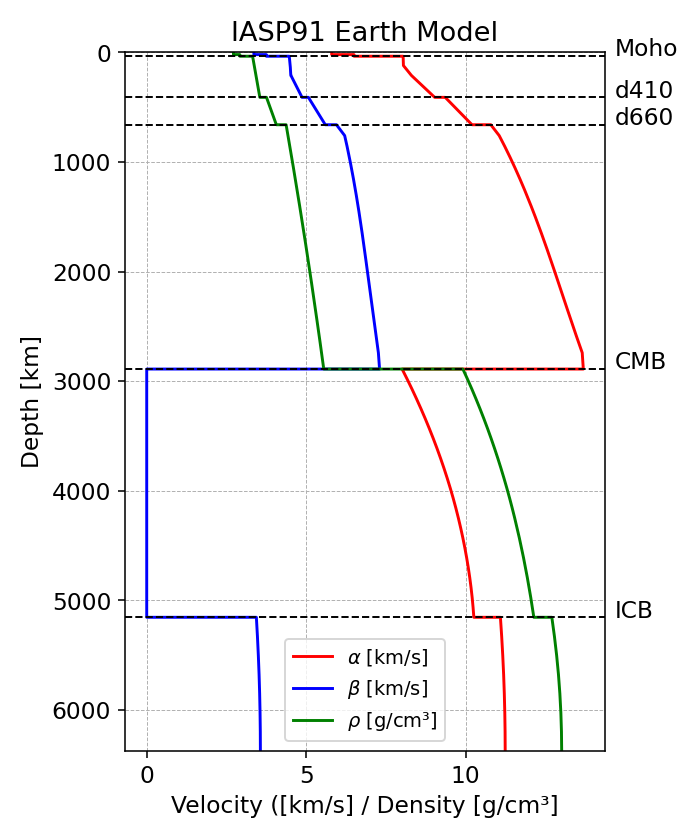
\includegraphics[width=0.8\textwidth]{figs/IASP91.png}
  \caption{The IASP91 Earth model displaying compressional wave velocity $\alpha$ (red), shear wave velocity $\beta$ (blue), and density $\rho$ (green) as functions of depth, with key discontinuities including the Moho, 410 km, 660 km, Core-Mantle Boundary (CMB), and Inner Core Boundary (ICB) marked.}
  \label{fig:iasp91}
\end{figure}

Compute travel times and ray paths for phases 'P' and 'S' at source depth 0 km and epicentral distance (delta) 20~$^{\circ}$. The ttimesAndPaths method returns a Phases object containing computed arrivals. Specifying phases limits computations to those; default is 'all'.

\begin{lstlisting}[language=Python]
phases = tracer.ttimesAndPaths(source_depth=0, delta=20, phases=['P', 'S'])
\end{lstlisting}

Print detailed information for all computed phases. The getInfo method displays a formatted table with phase name, travel time (ttime), take-off angle, dT/dD (ray parameter), and d2T/dD2 (second derivative for spreading).

\begin{lstlisting}[language=Python]
phases.getInfo()
\end{lstlisting}

Plot the ray paths for all computed phases. The plotPath method visualizes paths in a circular Earth section, with colored branches (e.g., P red, S blue, K orange) and black discontinuity circles. Source is yellow star, receiver red triangle.

\begin{lstlisting}[language=Python]
phases.plotPath()
\end{lstlisting}

\begin{figure}[H]
  \centering
  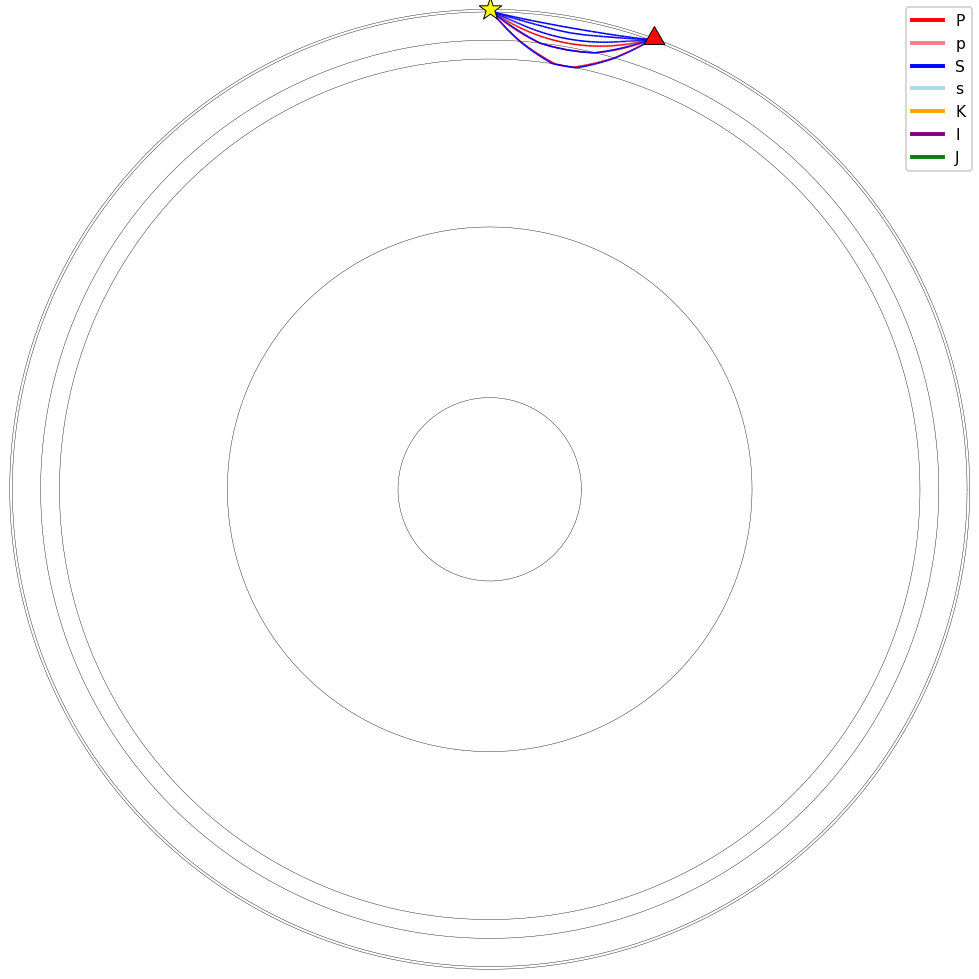
\includegraphics[width=0.8\textwidth]{figs/Regional_Ray_Paths.png}
  \caption{Ray paths for regional P (red) and S (blue) seismic phases from a surface source at an epicentral distance of 20°, illustrated in a cross-section of the Earth with discontinuity boundaries shown as concentric circles.}
  \label{fig:regional_ray_paths}
\end{figure}

Plot travel-time curves for default phases (`P' and `S'). The plotTravelTimes method generates curves of travel time (minutes) vs. delta (degrees), useful for understanding phase arrivals over distances.

\begin{lstlisting}[language=Python]
tracer.plotTravelTimes()
\end{lstlisting}

Compute diffracted phases `Pdiff' and `Sdiff' at delta 150~$^{\circ}$. Demonstrates handling of phases beyond the direct wave cutoff, extending along the CMB.

\begin{lstlisting}[language=Python]
phases = tracer.ttimesAndPaths(source_depth=0, delta=150, phases=['Pdiff', 'Sdiff'])
\end{lstlisting}

\begin{figure}[H]
  \centering
  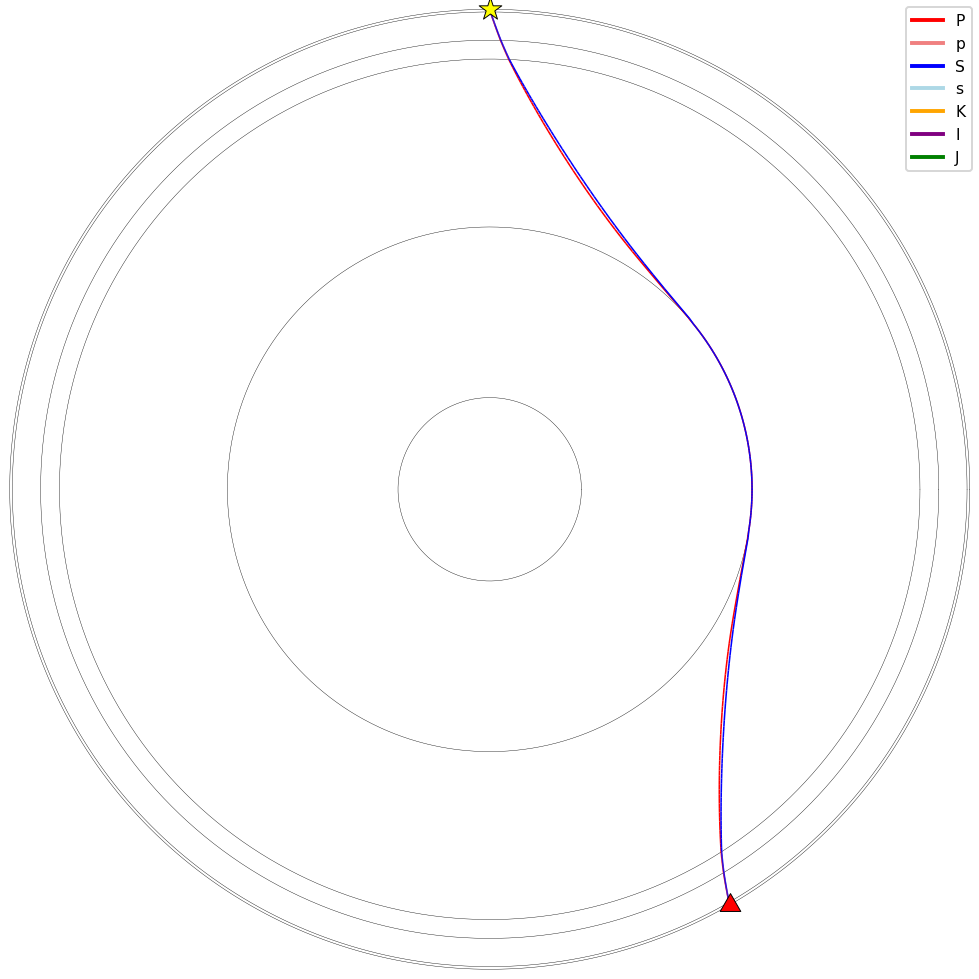
\includegraphics[width=0.8\textwidth]{figs/Diffraced_P_and_S_Rays.png}
  \caption{Ray paths for diffracted Pdiff (red) and Sdiff (blue) phases at an epicentral distance of 150°, showing waves grazing along the Core-Mantle Boundary (CMB) in the Earth's cross-section.}
  \label{fig:diffracted_p_and_s_rays}
\end{figure}

Plot travel-time curves including diffracted phases. Specifies phases to include both direct and diffracted for comparison.

\begin{lstlisting}[language=Python]
tracer.plotTravelTimes(phases=['P', 'S', 'Pdiff', 'Sdiff'])
\end{lstlisting}

Plot curves for a custom list of multiple phases, showcasing reflected, core, and converted phases.

\begin{lstlisting}[language=Python]
tracer.plotTravelTimes(phases=['PP', 'SS', 'PS', 'PKP', 'SKP', 'SKKS',
                               'PKIKP', 'PKIKS', 'PKJKP', 'SKS660t+P'])
\end{lstlisting}

\begin{figure}[H]
  \centering
  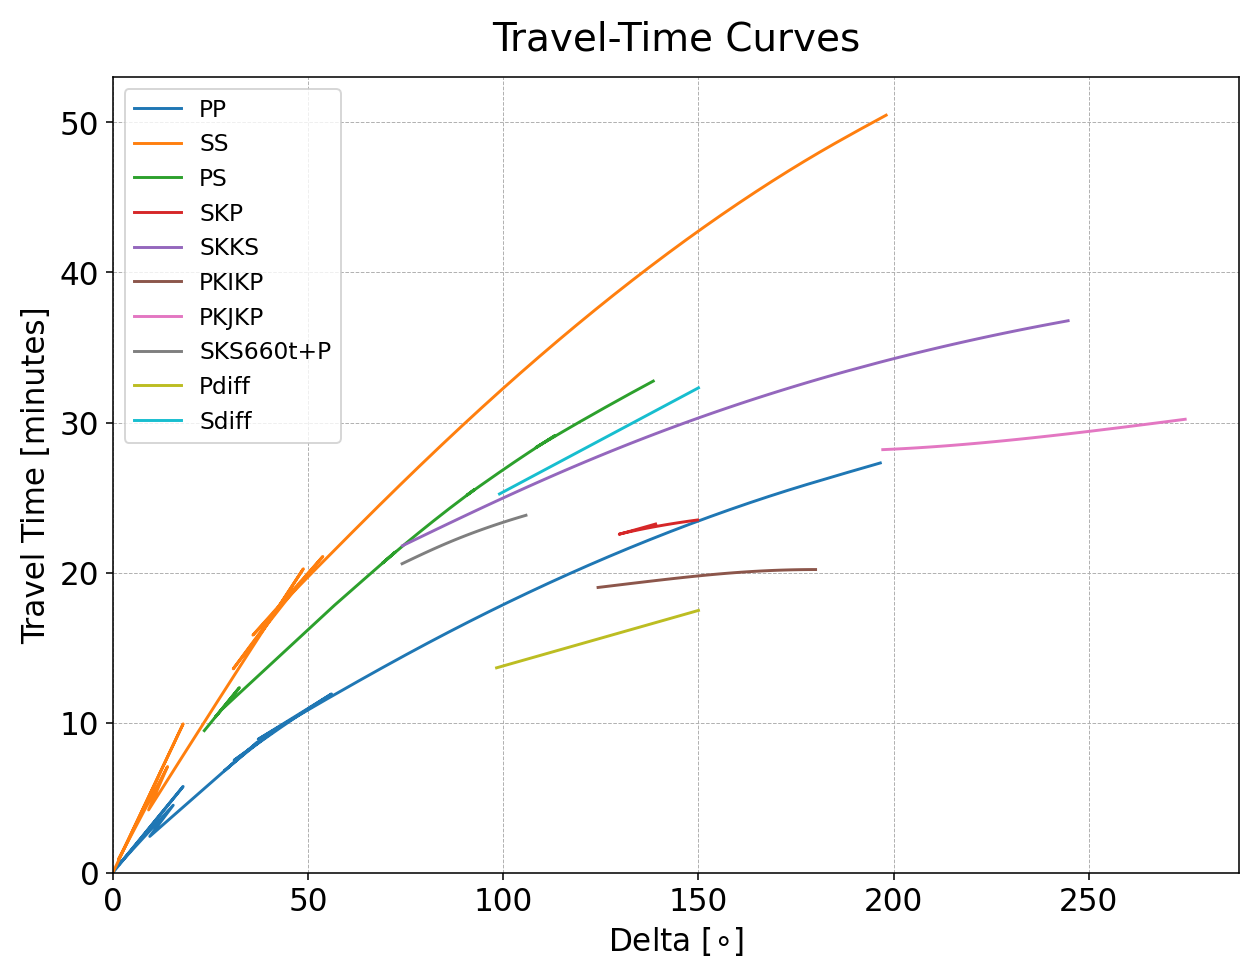
\includegraphics[width=0.8\textwidth]{figs/Travel_Time_Curves.png}
  \caption{Travel-time curves for multiple seismic phases including PP (blue), SS (orange), PS (green), PKP (red), SKP (purple), SKKS (brown), PKIKP (pink), PKIKS (gray), PKJKP (yellow), and SKS660t+P (cyan) as functions of epicentral distance Delta (°).}
  \label{fig:travel_time_curves}
\end{figure}

Plot amplitude coefficients at all discontinuities. Visualizes amplitude and energy flux vs. incidence angle for reflections/transmissions at each interface (e.g., surface, Moho).

\begin{lstlisting}[language=Python]
tracer.plotAmplitudeCoefficients(discontinuities='all')
\end{lstlisting}

\begin{figure}[H]
  \centering
  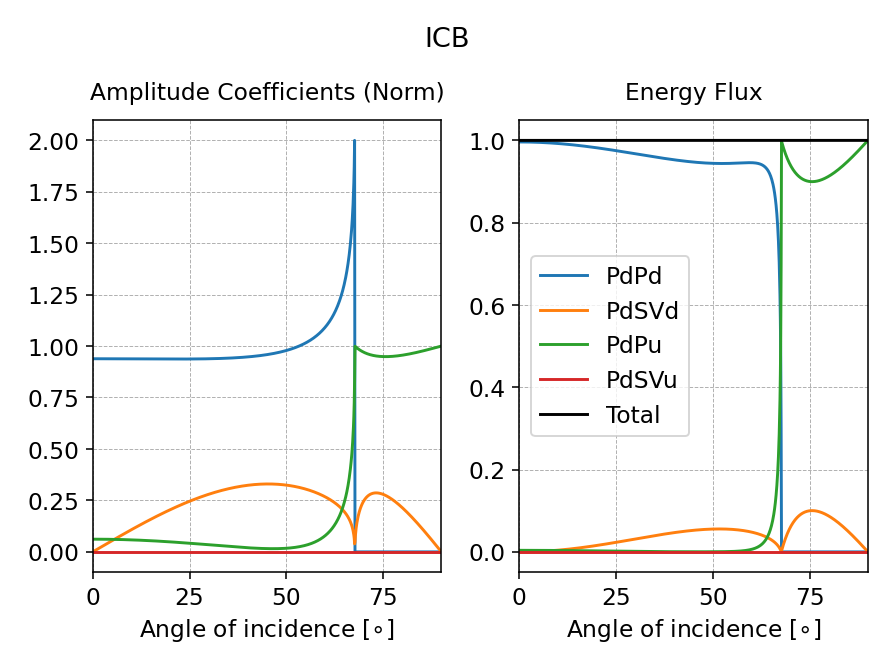
\includegraphics[width=0.8\textwidth]{figs/Amplitude_Coefficients_ICB.png}
  \caption{Normalized amplitude coefficients (left) and energy flux (right) at the Inner Core Boundary (ICB) versus angle of incidence, with curves for PdPd (blue), PdSvd (orange), PdPu (green), PdSvu (red), and total (black).}
  \label{fig:amplitude_coefficients_icb}
\end{figure}

Compute specific phases `P', `P410-P', and `SKS660t+P' at delta 98~$^{\circ}$, demonstrating phase naming for reflections and conversions.

\begin{lstlisting}[language=Python]
phases = tracer.ttimesAndPaths(source_depth=0, delta=98,
                               phases=['P', 'P410-P', 'SKS660t+P'])
\end{lstlisting}

Compute all minor-arc phases at depth 480 km and delta 140~$^{\circ}$.

\begin{lstlisting}[language=Python]
phases = tracer.ttimesAndPaths(source_depth=480, delta=140, arc='minor')
\end{lstlisting}

Compute all major-arc phases (counter-clockwise propagation).

\begin{lstlisting}[language=Python]
phases = tracer.ttimesAndPaths(source_depth=480, delta=140, arc='major')
\end{lstlisting}

Compute both minor and major arcs with amplitude computations enabled.

\begin{lstlisting}[language=Python]
phases = tracer.ttimesAndPaths(source_depth=480, delta=140, arc='both',
                               compute_amplitudes=True)
\end{lstlisting}

\begin{figure}[H]
  \centering
  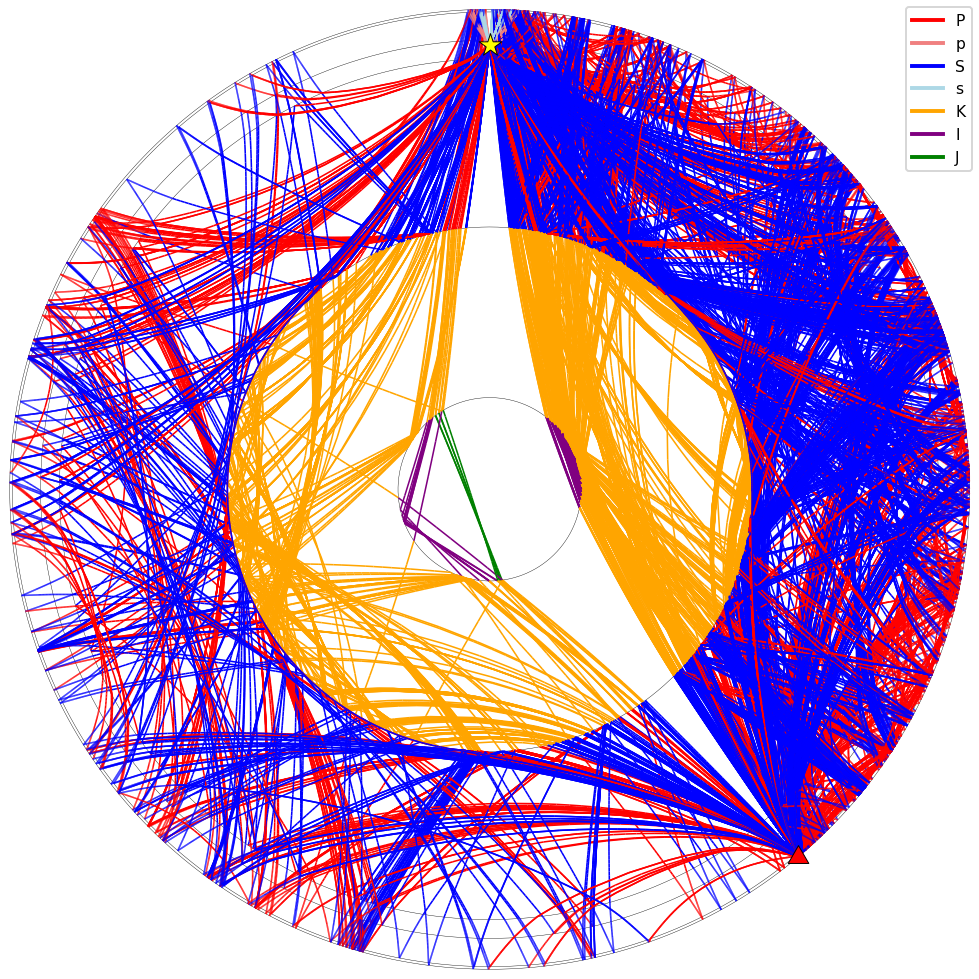
\includegraphics[width=0.8\textwidth]{figs/All_Ray_Paths.png}
  \caption{All available ray paths for seismic phases at a source depth of 20 km and epicentral distance of 150°, illustrating a dense network of wave propagations through the Earth's layers with color-coded branches.}
  \label{fig:all_ray_paths}
\end{figure}

Print info for selected phases from the computed set.

\begin{lstlisting}[language=Python]
phases.getInfo(['pPKJKS', 'P410-ScSScS'])
\end{lstlisting}

Retrieve ray path data (radii, deltas, branches) for a single phase as a dictionary, useful for further analysis or export.

\begin{lstlisting}[language=Python]
paths = phases.getPath(['pPKJKS'])
\end{lstlisting}

Retrieve all phase information (ttime, take-off, etc.) for a phase as a dictionary.

\begin{lstlisting}[language=Python]
phases_dict = phases.getDict(['pPKJKS'])
\end{lstlisting}

Plot paths for a list of specific complex phases.

\begin{lstlisting}[language=Python]
phases.plotPath(['PKIIKP', 'PKP660t+SScP', 'PKJKS',
                 'SPS660-S', 'ScSScS660-ScS_M', 'pPKJKS',
                 'pPmt-ScSScS', 'P410-ScSScS', 'sSKIKPPm+P'])
\end{lstlisting}

\begin{figure}[H]
  \centering
  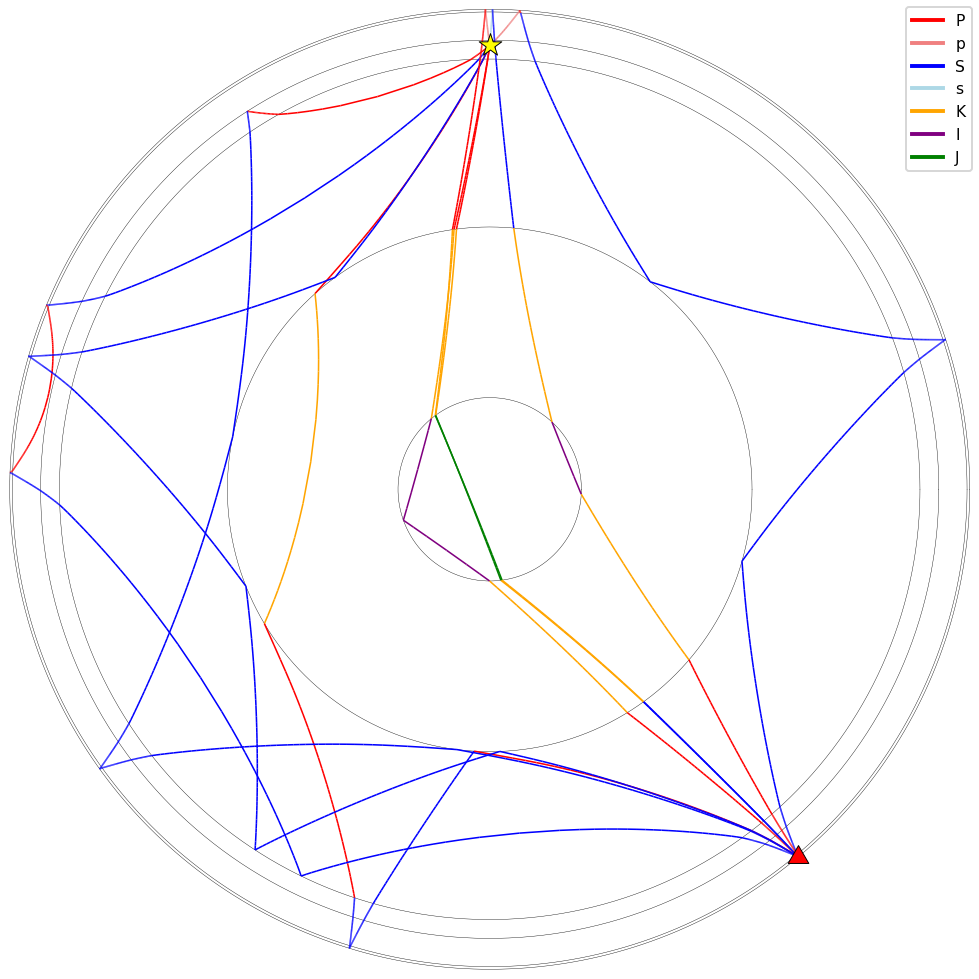
\includegraphics[width=0.8\textwidth]{figs/Selected_Ray_Paths.png}
  \caption{Selected ray paths for complex seismic phases including PKIIKP, PKP660t+SScP, PKJKS, SPS660-S, ScSScS660-ScS\_M, pPKJKS, pPmt-ScSScS, P410-ScSScS, and sSKIKPPm+P, color-coded by branch type (P red, S blue, K orange, J purple, I green) in the Earth's cross-section.}
  \label{fig:selected_ray_paths}
\end{figure}

Compute minor-arc phases including higher-order multiples up to 2 loops (e.g., for long-distance multiples).

\begin{lstlisting}[language=Python]
phases = tracer.ttimesAndPaths(source_depth=480, delta=140, arc='minor',
                               min_loop=0, max_loop=2)
\end{lstlisting}

\begin{figure}[H]
  \centering
  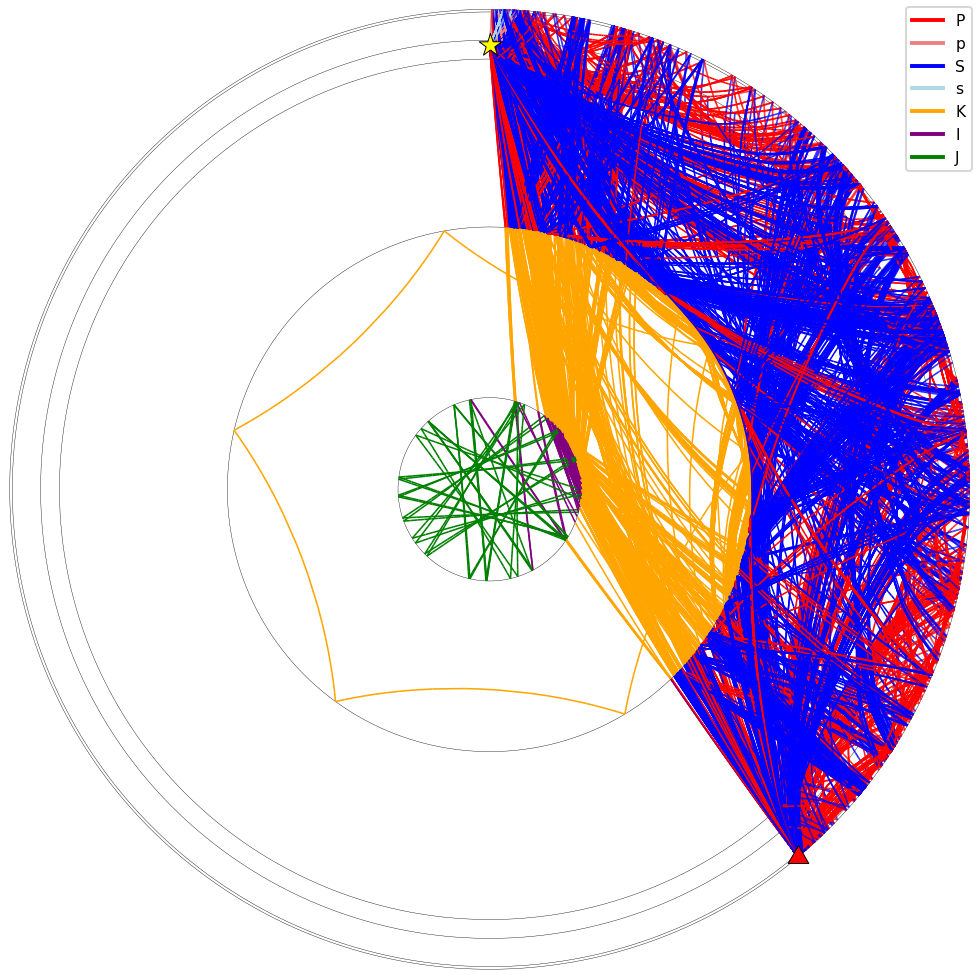
\includegraphics[width=0.8\textwidth]{figs/Higher_Order_Ray_Paths.png}
  \caption{Higher-order ray paths for seismic phases with up to 2 loops in the minor arc at a source depth of 480 km and epicentral distance of 140°, displaying multiple reflections and conversions in the Earth's interior.}
  \label{fig:higher_order_ray_paths}
\end{figure}

Compute all available phases at depth 20~km and delta 150~$^{\circ}$.

\begin{lstlisting}[language=Python]
phases = tracer.ttimesAndPaths(source_depth=20, delta=150)
\end{lstlisting}

\section{Phase naming convention}

The standard IASPEI phase list \parencite{Storchak2003,Storchak2011} is insufficient to uniquely label all the paths produced by the binary-tree algorithm of \texttt{SeisTracer}, particularly when uncommon mode conversions, deep multiples, and repeated core legs are included. The package therefore implements a flexible naming convention that follows the IASPEI standard where applicable and extends it as needed. The convention is summarized below.

Each ray path is internally represented as a sequence of the propagation-leg keys Pu, Pd, Su, and Sd. These keys are mapped automatically to the standard phase letters
\begin{itemize}
  \item P/p for compressional waves in the mantle (and the mantle leg of a teleseismic phase),
  \item S/s for shear waves in the mantle,
  \item K for the outer core (compressional),
  \item I for the inner core (compressional),
  \item J for the inner core (shear).
\end{itemize}
The first letter is written in lowercase (p or s) when the initial leg leaves the source upgoing, and uppercase (P or S) otherwise.

Discontinuity labels are appended to indicate the location of reflections and conversions: m for the Moho, 410 and 660 for the upper-mantle discontinuities, c for the CMB, and i for the ICB. Two additional symbols qualify the interaction at a discontinuity:
\begin{itemize}
  \item ``+'' indicates a reflection from the inner side of the discontinuity (i.e., the wave approaches from below);
  \item ``-'' indicates a reflection from the outer side (the wave approaches from above);
  \item ``t'' indicates a wave that undergoes a mode conversion during transmission through the discontinuity rather than a reflection at it.
\end{itemize}

When both minor- and major-arc phases are requested, the suffixes ``\_m'' and ``\_M'' disambiguate them.

As an example, the phase \texttt{PSP410t-S} corresponds to a ray that leaves the source as a downgoing P wave, reflects at the surface as an S wave, reflects again at the surface converting back to P, and finally undergoes a mode conversion to S during transmission through the 410-km discontinuity before arriving at the receiver. The convention provides a compact yet unambiguous description of even the most complex ray paths produced by \texttt{SeisTracer}.

For contributions or issues, contact the author.
\end{document}
